\part{Metody pro odhad tvaru kamene}

\section{Triangulace, polarizace a profilprojektor}
	3D rekonstrukce objektů je častá úloha počítačového vidění. Existuje řada sofistikovaných metod, které z~více pohledů kamer vytvoří model objektu s vysokou přesností. Většina z~po\-u\-ží\-va\-ných algoritmů není použitelná pro průhledné objekty, jako je broušený kámen. Pro odhad tvaru broušeného kamene musíme použít specializované metody, které uvažují zákony lomu a odrazu či polarizaci světla. 
	
	Kutulakos et al. \cite{Kutulakos2008} přichází s myšlenkou triangulace cesty světelného paprsku. Cestu definují pozice zdrojů světla, odrazy či lomy od rozhraní a pozice kamer. Ukazuje, za jakých podmínek lze vypočítat pozice dopadu paprsku na rozhraní zároveň s normálou tohoto elementu. 
	 
	 Miyazaki a Ikeuchi \cite{PolarTrace} vyhodnocují polarizace odraženého světla od měřeného objektu. Model objektu je určen na základě Fresnelových rovnic \cite{Handbook}. Toto měření je zdlouhavé a vyžaduje složité měřicí zařízení.    


  Pro měření a vyhodnocení brusu diamantů se komerčně využívají produkty firmy Sarine \cite{Sarine}. Optická cesta je uspořádána jako profilprojektor tzn. zdroj kolimovaného světla, kámen, kamera. Kámen se při měření otáčí okolo vertikální osy. Otáčením kamene získáme sérii mnoha snímků. Vyhodnocením snímků získáme model kaneme. 
\begin{figure}[h!]
     \centering 
     \adjincludegraphics[height=5cm,trim={0 {.2\height} 0  {.2\height}},clip]{sarin.jpg}
     %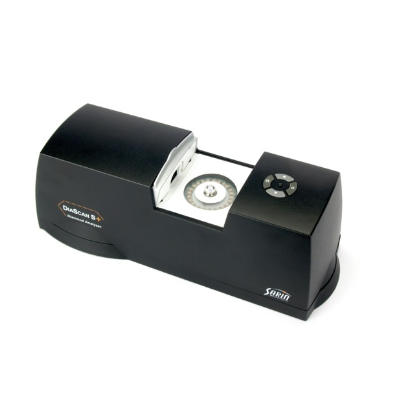
\includegraphics[height =5cm]{sarin.jpg} 

\caption[Sarine Diascan S+.]{Sarine Diascan S+. Převzato z \cite{DiaScan}.}

\label{fig:histogram relativni pohyb }

\end{figure}
  
\newpage
\section{Předchozí práce}

\paragraph{LADOK}
\hspace{1mm}

Základním nástrojem dlouhodobého výzkumu v Centru strojového vnímání na katedře kybernetiky Elektrotechnické fakulty ČVUT při zkoumání broušených kamenů je software LADOK \cite{Pohl2002} od Petra Pohla. Simulační program LADOK zavádí pro broušený kámen ge\-o\-me\-tri\-cký model ve formě konvexního mnohostěnu. Na povrch kamene dopadá svazek rovnoběžných paprsků světla homogenní intenzity a známého směru. LADOK simuluje odrazy, lomy a dělení svazků na povrchu kamene. Svazky po opuštění kamene mají známý směr, zářivý tok, plochu a tvar. Tento software rozšířil Igor Bodlák \cite{bodlakLADOK} o výpočet polarizace. Matematický model kamene obohatil Martin Straka \cite{strakaLADOK}. Přechody mezi fasetami modeloval jako posloupnost většího počtu menších faset. 

Software LADOK simuluje experiment na obr. \ref{fig:basicMeasure}. V tomto experimentu je zdrojem světla laser. Laserový svazek dopadá na broušený kámen, kde se roztříští na mnoho menších svazků. Ty jsou po opuštění kamene zachyceny na stínítku. Stínítko snímáme kamerou a získáváme obraz svazků na stínítku ve formě digitálního obrazu.  


\begin{figure}[h!]
\begin{center}
\scalebox{0.5}{ \input{xfig/stinitko.pstex_t}}
\end{center}
\caption[Schéma experimentu.]{Nákres principu experimentu. Laser produkuje svazek světla, který dopadá na celou plochu kamene. V kameni se svazek rozdělí na mnoho svazků. Svazky vystupující z kamene v horní polorovině dopadnou na stínítko. Stínítko snímá kamera. Převzato z \cite{Drapela}.}
\label{fig:basicMeasure}
\end{figure}

\newpage
\paragraph{Měřicí soustava}
\hspace{1mm}

Experimentální soustavu máme sestavenou (obr. \ref{fig: merici soustava}) a zkalibrovanou \cite{Drapela}. Výstupem experimentu je snímek s obrazy svazků. Všechny příklady snímků v této práci jsou vykresleny v invertované podobě. Z \cite{Drapela} známe transformaci mezi obrazem svazku na stínítku a směrem, ve kterém opouští kámen. 

\begin{figure}[h!]
    \centering
    \begin{minipage}[c]{0.50\textwidth}
        \centering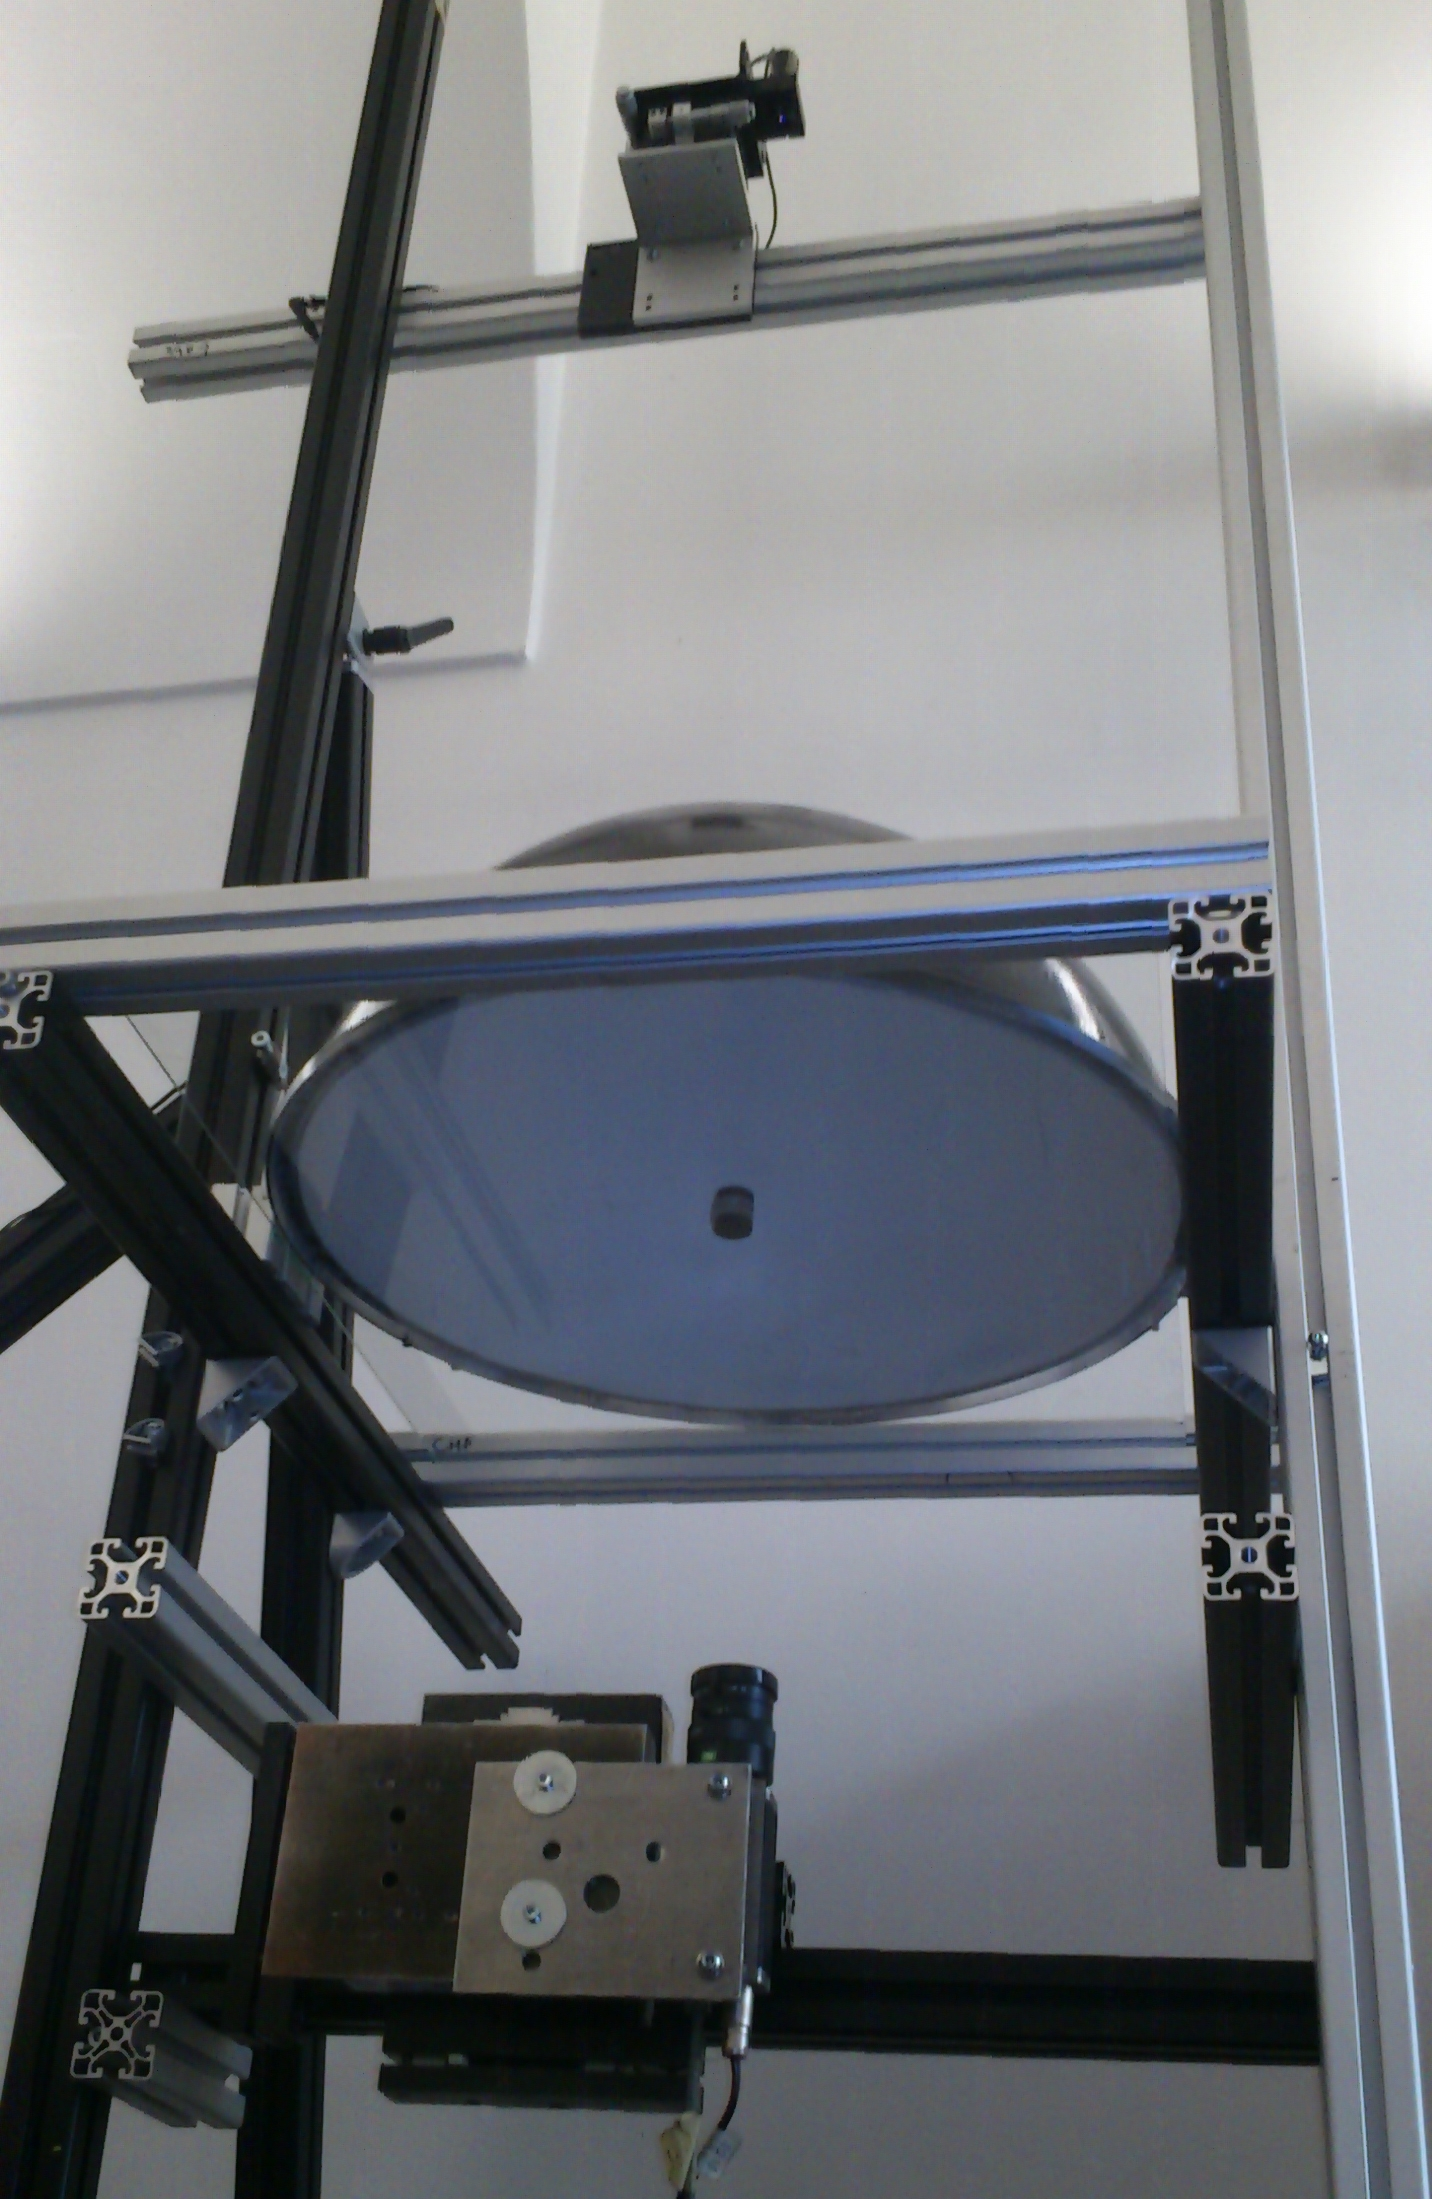
\includegraphics[height = 12cm]{soustava2.jpg}
    \end{minipage}
    \begin{minipage}[c]{0.46\textwidth}
        \centering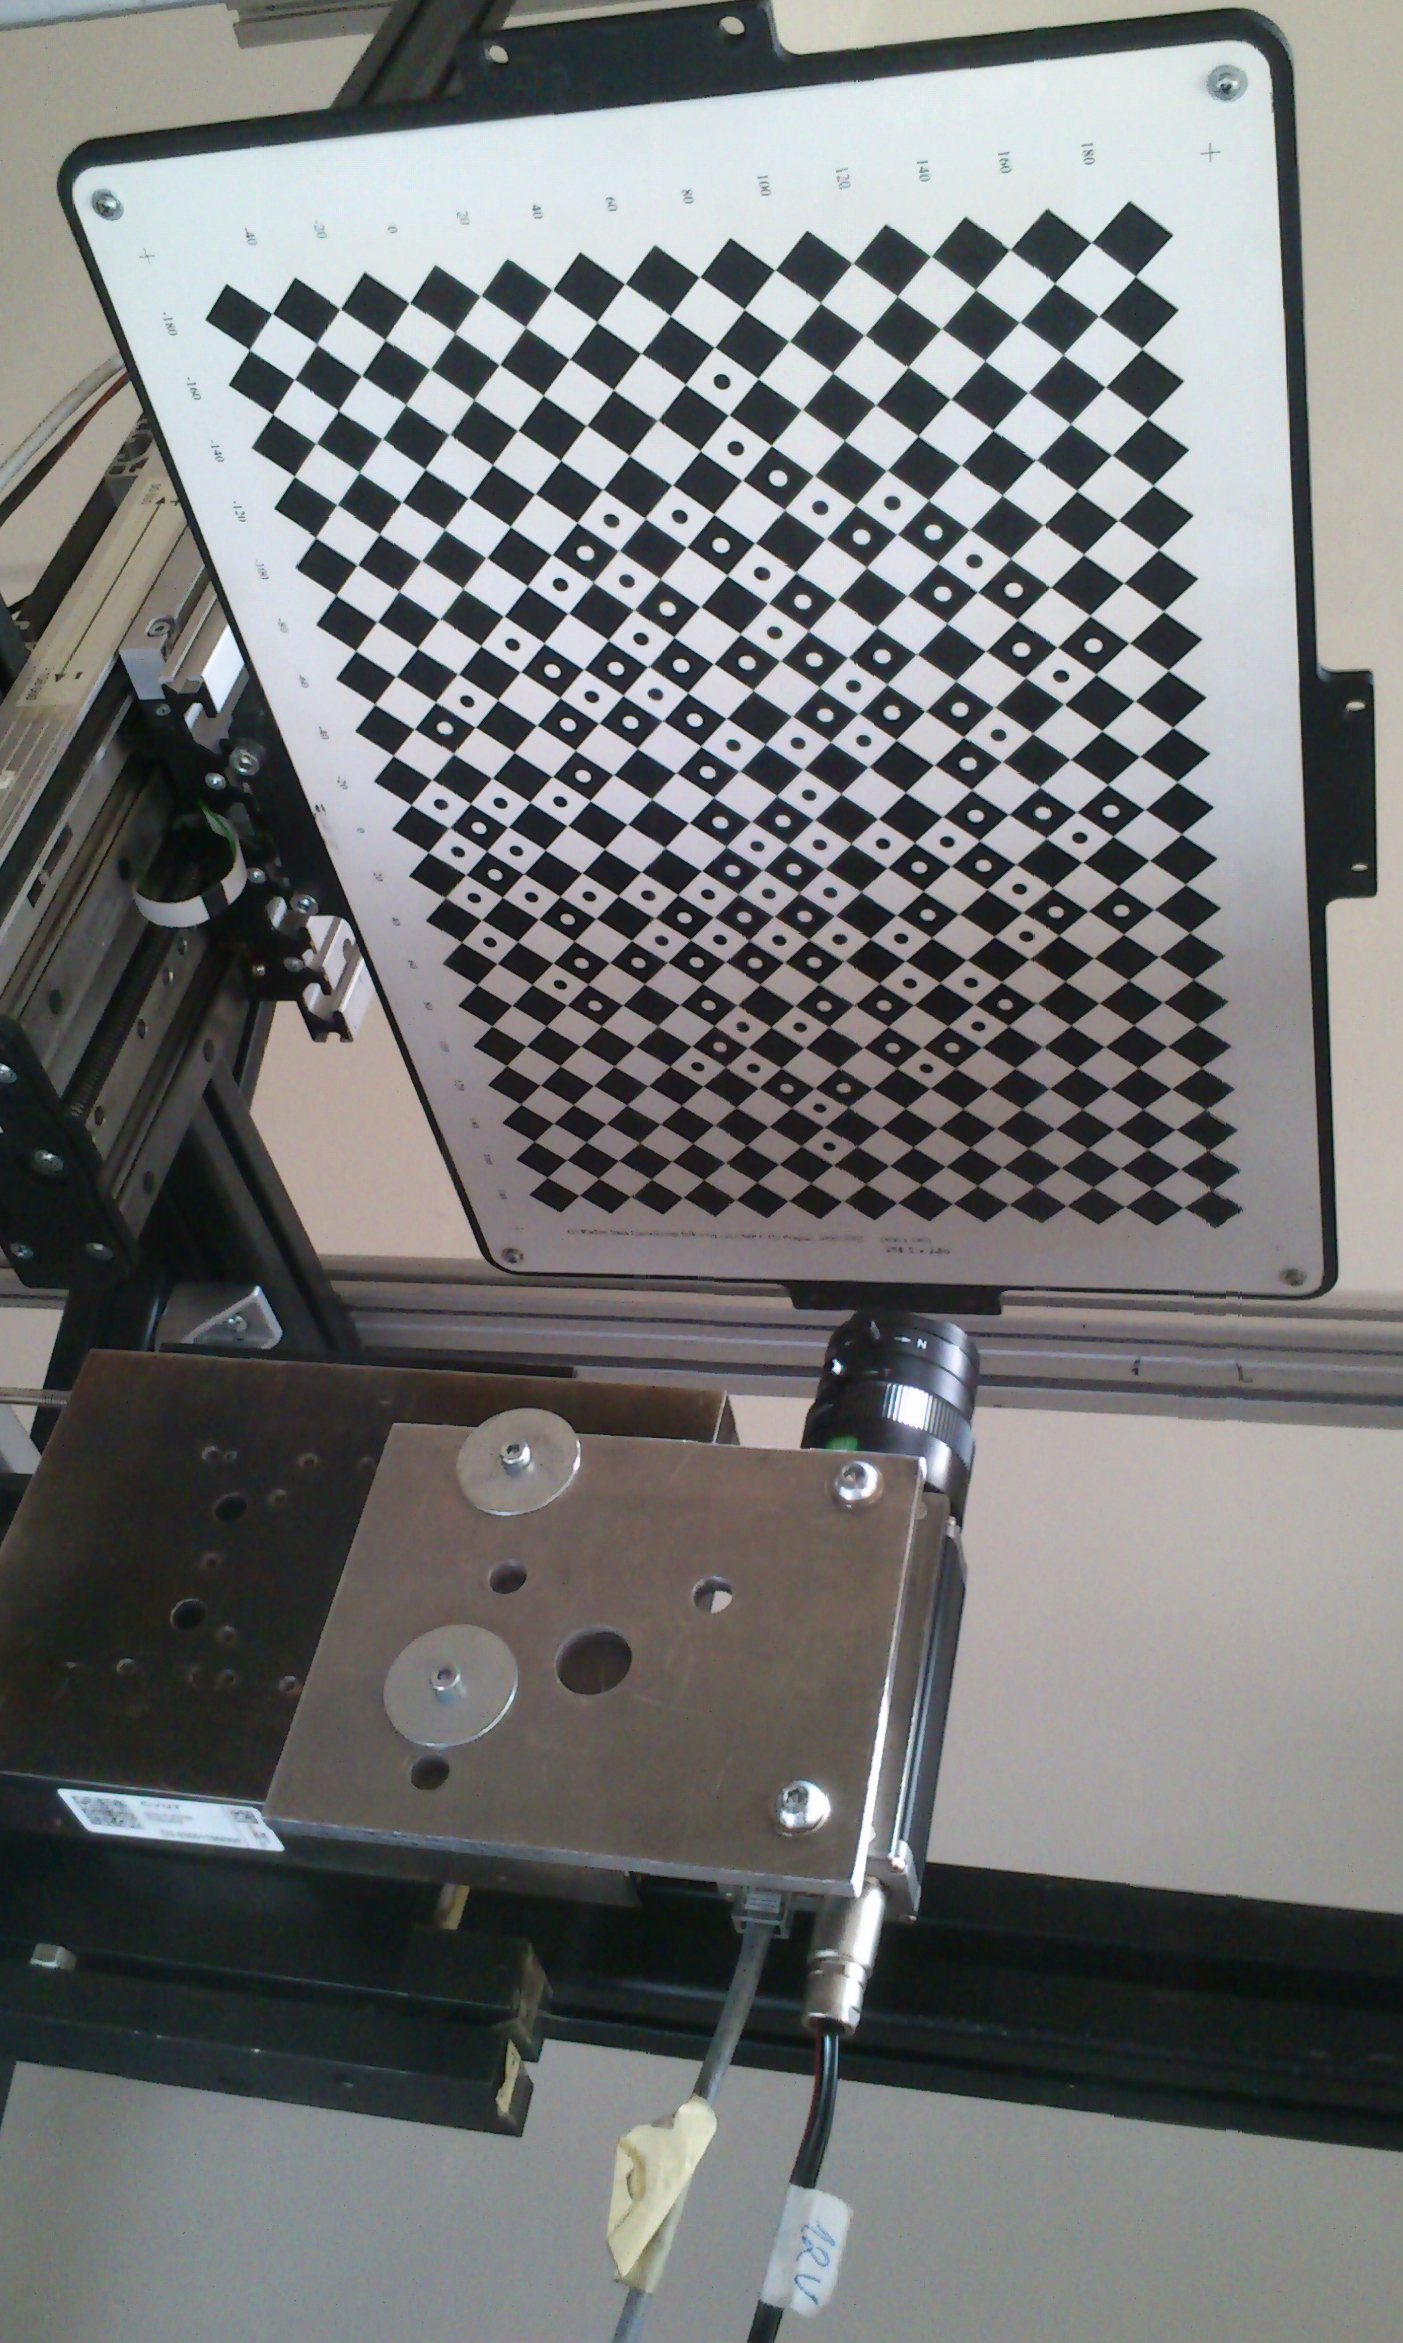
\includegraphics[height = 12cm]{kalib_obrazec.jpg}
    \end{minipage}
    \\
        \caption[Měřicí soustava.]{Experimentální soustava pro zachycení svazků vycházejících z kamene ozářeného laserovým svazkem. Vlevo: sestavená měřicí soustava. Zdroj laserového svazku je umístěn v horní části. Laserový svazek prochází otvorem ve stínítku a dopadá na kámen položený na podstavci. Svazky vycházející z kamene v horní polorovině dopadnou na půlkulové stínítko. Podstavec a stínítko jsou položeny na skleněné tabuli. Obraz stínítka snímá kamera. Vpravo: sestavení soustavy při kalibraci kamery. Převzato z \cite{Drapela}.}
    \label{fig: merici soustava}
\end{figure}

\newpage
\paragraph{LAM}
\hspace{1mm}

Igor Bodlák \cite{Bodlak2005} umožnil porovnání dat reálného experimentu s výsledky počítačové simulace. Navrhl optimalizaci kritéria hodnotící rozdíl vzdálenosti stop z experimentu a odrazů stop simulace na stínítku. Optimalizovaly se parametry faset kamene a kámen se tak deformoval, aby se dosáhlo co nejlepší shody v zadaném kritériu. Software pro řešení inverzní úlohy nazval zkratkou LAM. 

LAM byl použitelný pouze pro broušený kámen čtvercového tvaru. Z důvodu složitosti přiřazení stop z experimentu k obrazům simulovaných svazků při osvětlení celého kamene se v LAMu zaměřil  vstupní laserový svazek pouze do určitých míst kamene. Tím vzniklo redukované množství svazků a korespondence se simulovanými svazky se výrazně zjednodušila. Nevýhodou tohoto přístupu jsou rozměry kamene, které musí být několikanásobně větší než průměr laserového svazku. Metoda je prakticky nepoužitelná pro kameny o rozměrech v jednotkách milimetru. 

\paragraph{Příspěvek práce} 
\hspace{1mm}

 	V této práci osvítíme laserovým svazkem celý kámen. Zaměříme se na kameny šatonové růže s plochým spodkem a 12 bočními fasetami. Tyto kameny se ve zkratce nazývají \textit{viva12}. Rozměry kamenů budou v řádech milimetrů. 
	
	K robustní detekci obrazu svazků z digitálního obrazu použijeme MSER detektor \cite{Matas}. Z~výsledku detekce určíme parametry stop. Sestavíme program, pomocí kterého bude možno manuálně párovat obrazy svazků broušeného kamene se simulovanými stopami.
	
 Optimalizací z~LAMu získáme náklony faset. Parametry svazků prozkoumáme pomocí cílených experimentů. Navrhneme algoritmus pro \textit{vivu12}, který určí automaticky orientaci faset kamene. Výstupem programu budou odchylky úhlů faset kamene od jejich ideální pozice.




 
 
 
 \clearpage
 